% \begin{figure}[ht]
%      \centering
%      \begin{subfigure}{0.9\linewidth}
%      \centering
%             \begin{tikzpicture}
%             \tikzstyle{vertex}=[circle,fill=none,draw=black,minimum size=17pt,inner sep=0pt]
% \node[vertex] (S) at (0,0) {$S$};
% \node[vertex] (A) at (2,0) {$A$};
% \node[vertex] (D) at (1,1) {$D$};
% \path (S) edge (D);
% \path (D) edge (A);
% \path[red] (S) edge (A);
%             \end{tikzpicture}
%         \caption{Causal graph for $\model \in \modelsunconfedge$ illustrating all possible functional dependencies.}
%         \label{fig:no-cf-edge}
%         \end{subfigure}    \hfill
% %              \begin{subfigure}{0.45\linewidth}
% %              \centering
% %             \begin{tikzpicture}
% %             \tikzstyle{vertex}=[circle,fill=none,draw=black,minimum size=17pt,inner sep=0pt]
% % \node[vertex] (S) at (0,0) {$S$};
% % \node[vertex] (A) at (2,0) {$A$};
% % \node[vertex] (D) at (1,1) {$D$};
% % \path (S) edge (D);
% % \path (D) edge (A);
% % %\path[red] (S) edge (A);
% %             \end{tikzpicture}
% %         \caption{Causal graph for $\model \in \nullgraphunconf$ illustrating all possible functional dependencies.}
% %         \label{fig:no-cf-no-edge}
% %         \end{subfigure}
% \end{figure}

% \begin{figure}[h]
%      \centering
%             \begin{tikzpicture}
%             \tikzstyle{vertex}=[circle,fill=none,draw=black,minimum size=17pt,inner sep=0pt]
% \node[vertex] (S) at (0,0) {$S$};
% \node[vertex] (A) at (2,0) {$A$};
% \node[vertex] (D) at (1,1) {$D$};
% \path (S) edge (D);
% \path (D) edge (A);
% \path[bidirected] (D) edge[bend left=60] (A);
% \path[red] (S) edge (A);
% % \draw[->, line width=0.3mm]  (S)--(D);
% % \draw[->, line width=0.3mm]  (D)--(A);
% % \draw[->, line width=0.3mm]  (S)--(A);
% % \draw[<->, line width=0.3mm]  (D)--(A);
%             \end{tikzpicture}
%         \caption{Causal graph for $\model \in \modelsunconfedge$ illustrating all possible functional dependencies.}
%         \label{fig:cf-no-edge}
% \end{figure}

% \begin{figure}[h]
%      \centering
%             \begin{tikzpicture}
%             \tikzstyle{vertex}=[circle,fill=none,draw=black,minimum size=17pt,inner sep=0pt]
% \node[vertex] (S) at (0,0) {$S$};
% \node[vertex] (A) at (3,-0.5) {$A$};
% \node[vertex] (D) at (1,1) {$D$};
% \node[vertex] (S') at (1,-0.5) {$S'$};
% \path (S) edge (D);
% \path (D) edge (A);
% \path[bidirected] (D) edge[bend left=60] (A);
% \path[red] (S') edge (A);
% %\path (S) edge (S'); 
%  \path (S) edge node[near start, below] {=} (S');
% % \draw[->, line width=0.3mm]  (S)--(D);
% % \draw[->, line width=0.3mm]  (D)--(A);
% % \draw[->, line width=0.3mm]  (S)--(A);
% % \draw[<->, line width=0.3mm]  (D)--(A);
%             \end{tikzpicture}
%         \caption{Causal graph for $\model \in \modelsedge$ illustrating all possible functional dependencies.} 
%         \label{fig:cf-edge}
% \end{figure}


%              \begin{subfigure}{0.45\linewidth}
%              \centering
%             \begin{tikzpicture}
%             \tikzstyle{vertex}=[circle,fill=none,draw=black,minimum size=17pt,inner sep=0pt]
% \node[vertex] (S) at (0,0) {$S$};
% \node[vertex] (A) at (2,0) {$A$};
% \node[vertex] (D) at (1,1) {$D$};
% \path (S) edge (D);
% \path (D) edge (A);
% %\path[red] (S) edge (A);
%             \end{tikzpicture}
%         \caption{Causal graph for $\model \in \nullgraphunconf$ illustrating all possible functional dependencies.}
%         \label{fig:no-cf-no-edge}
%         \end{subfigure}
%\end{figure}

\begin{figure*}[t]
     \centering
     \begin{subfigure}{0.32\linewidth}
     \centering
            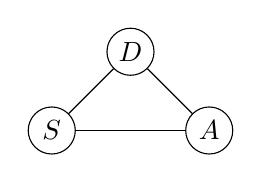
\begin{tikzpicture}
            \tikzstyle{vertex}=[circle,fill=none,draw=black,minimum size=17pt,inner sep=0pt]
\node[vertex] (S) at (0,0) {$S$};
\node[vertex] (A) at (2,0) {$A$};
\node[vertex] (D) at (1,1) {$D$};
\path (S) edge (D);
\path (D) edge (A);
\path (S) edge (A);
            \end{tikzpicture}
        \caption{$\model \in \modelsunconfedge$}
        \label{fig:no-cf-edge}
\end{subfigure}
     \begin{subfigure}{0.32\linewidth}
     \centering
            \begin{tikzpicture}
            \tikzstyle{vertex}=[circle,fill=none,draw=black,minimum size=17pt,inner sep=0pt]
\node[vertex] (S) at (0,0) {$S$};
\node[vertex] (A) at (2,0) {$A$};
\node[vertex] (D) at (1,1) {$D$};
%\node[vertex] (S') at (1,-0.5) {$S'$};
\path (S) edge (D);
\path (D) edge (A);
\path[bidirected] (D) edge[bend left=60] (A);
\path (S) edge (A);
%\path (S) edge (S'); 
% \path (S) edge node[near start, below] {=} (S');
% \draw[->, line width=0.3mm]  (S)--(D);
% \draw[->, line width=0.3mm]  (D)--(A);
% \draw[->, line width=0.3mm]  (S)--(A);
% \draw[<->, line width=0.3mm]  (D)--(A);
            \end{tikzpicture}
        \caption{$\model \in \modelsedgerelax$} 
        \label{fig:cf-edge}
        \end{subfigure}
         \begin{subfigure}{0.32\linewidth}
     \centering
            \begin{tikzpicture}
            \tikzstyle{vertex}=[circle,fill=none,draw=black,minimum size=17pt,inner sep=0pt]
\node[vertex] (S) at (0,0) {$S$};
\node[vertex] (A) at (2,0) {$A$};
\node[vertex] (D) at (1,1) {$D$};
%\node[vertex] (S') at (1,-0.5) {$S'$};
\path (S) edge (D);
\path (D) edge (A);
\path[bidirected] (D) edge[bend left=60] (A);
%\path (S) edge (A);
%\path (S) edge (S'); 
% \path (S) edge node[near start, below] {=} (S');
% \draw[->, line width=0.3mm]  (S)--(D);
% \draw[->, line width=0.3mm]  (D)--(A);
% \draw[->, line width=0.3mm]  (S)--(A);
% \draw[<->, line width=0.3mm]  (D)--(A);
            \end{tikzpicture}
        \caption{$\model \in \nullgraph$ and $\model \in \modeliv$} 
        \label{fig:cf-edge-iv}
        \end{subfigure}
        \caption{Causal graphs, $\cg{\model}$, assumed in various model classes.}
\end{figure*}

% \begin{figure}
%      \centering
%             \begin{tikzpicture}
%             \tikzstyle{vertex}=[circle,fill=none,draw=black,minimum size=17pt,inner sep=0pt]
% \node[vertex] (Z) at (0,0) {$Z$};
% \node[vertex] (Y) at (3,0) {$Y$};
% \node[vertex] (X) at (1.5,0) {$X$};
% %\node[vertex] (S') at (1,-0.5) {$S'$};
% \path (Z) edge (X);
% \path (X) edge (Y);
% \path[bidirected] (X) edge[bend left=60] (Y);
% %\path[red] (S') edge (A);
% %\path (S) edge (S'); 
%  %\path (S) edge node[near start, below] {=} (S');
% % \draw[->, line width=0.3mm]  (S)--(D);
% % \draw[->, line width=0.3mm]  (D)--(A);
% % \draw[->, line width=0.3mm]  (S)--(A);
% % \draw[<->, line width=0.3mm]  (D)--(A);
%             \end{tikzpicture}
%         \caption{Causal graph of $M \in \modeliv$} 
%         \label{fig:iv}
%         \end{figure}